\documentclass[11pt,A4]{article}

%\usepackage{charter}
%\usepackage[charter]{mathdesign}
\usepackage{ethminutes}
\usepackage{bstnotations}
\usepackage{tikz}

%\usepackage[english]{babel}
\selectlanguage{english}
\graphicspath{{./},{./Figures/}}
\renewcommand{\baselinestretch}{1.3}

\begin{document}
%---------------------------------------------------------------------
%     Properties of the document
%--------------------------------------------------------------------- 
\RefDocument{Thesis-Name-001}
\Date{March 11th, 2013}
\LieuReunion{UQ Chair}
\Redacteur{Ph.D student}     
\TitleReport{Ph.D thesis progress meeting}
\DateDiffusion{--} 
\Destinataires{B. Sudret} 

\entete
\pieddepage 
\PageDeGarde

\vspace*{2em}


%%% Actions
 \begin{table}[!ht]
    \centering
 \begin{tabularx}{\textwidth}{>{\lratio{0.3}\raggedright\arraybackslash}Y
      >{\lratio{1}\raggedright\arraybackslash}Y   >{\lratio{0.2}}Y}
    
      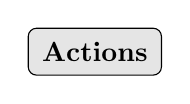
\begin{tikzpicture} 
        \draw (0,0) node[fill=black!10!white, draw=black, rectangle, text
        centered, rounded corners = 3pt,inner sep= 5pt] (Participants)
        {\bf Actions};
      \end{tikzpicture} \\[-0.3em] \toprule {\bf Responsable} & {\bf
        Action} & {\bf Deadline} \\\hline 
    Your Name & Description of the action& dd/mm/year\\ \bottomrule
    \end{tabularx}
  \end{table}

\newpage


%---------------------------------------------------------------------
%     Main text
%---------------------------------------------------------------------

\section{First section}
\subsection{Subsection}
\subsubsection{Subsubsection}

TARATATA 

Lorem ipsum dolor sit amet, consectetur adipiscing elit. Sed non risus.
Suspendisse lectus tortor, dignissim sit amet, adipiscing nec, ultricies


sed, dolor. Cras elementum ultrices diam. Maecenas ligula massa, varius
a, semper congue, euismod non, mi. Proin porttitor, orci nec nonummy
molestie, enim est eleifend mi, non fermentum diam nisl sit amet erat.
Duis semper. Duis arcu massa, scelerisque vitae, consequat in, pretium
a, enim. Pellentesque congue. Ut in risus volutpat libero pharetra
tempor. Cras vestibulum bibendum augue. Praesent egestas leo in pede.
Praesent blandit odio eu enim. Pellentesque sed dui ut augue blandit
sodales. Vestibulum ante ipsum primis in faucibus orci luctus et
ultrices posuere cubilia Curae; Aliquam nibh. Mauris ac mauris sed pede
pellentesque fermentum. Maecenas adipiscing ante non diam sodales
hendrerit. Ut velit mauris, egestas sed, gravida nec, ornare ut, mi.
Aenean ut orci vel massa suscipit pulvinar. Nulla sollicitudin. Fusce
varius.



\begin{equation}
  \label{eq:001}
  E = mc^2
\end{equation}

Ligula non tempus aliquam, nunc turpis ullamcorper nibh, in
tempus sapien eros vitae ligula. Pellentesque rhoncus nunc et augue.
Integer id felis. Curabitur aliquet pellentesque diam. Integer quis
metus vitae elit lobortis egestas. Lorem ipsum dolor sit amet,
consectetuer adipiscing elit. Morbi vel erat non mauris convallis
vehicula. Nulla et sapien. Integer tortor tellus, aliquam faucibus,
convallis id, congue eu, quam. Mauris ullamcorper felis vitae erat.
Proin feugiat, augue non elementum posuere, metus purus iaculis lectus,
et tristique ligula justo vitae magna. Aliquam convallis sollicitudin
purus. Praesent aliquam, enim at fermentum mollis, ligula massa
adipiscing nisl, ac euismod nibh nisl eu lectus. Fusce vulputate sem at
sapien. Vivamus leo. Aliquam euismod libero eu enim. Nulla nec felis sed
leo placerat imperdiet. Aenean suscipit nulla in justo. Suspendisse
cursus rutrum augue. Nulla tincidunt tincidunt mi. Curabitur iaculis,
lorem vel rhoncus faucibus, felis magna fermentum augue, et ultricies
lacus lorem varius purus. Curabitur eu amet.


%%%
\subsection{Table}
This is a sample table referred to as Table~\ref{tab:001}.


\begin{table}[!ht]
  \begin{center}      \caption{Exemple de table} \label{tab:001}
    \begin{tabularx}{\textwidth}
      {>{\lratio{0.9}}Y>{\lratio{0.9}}Y>{\lratio{0.9}}Y>{\lratio{1.3}}Y}
      \hline \rowcolor[gray]{0.98} {Parameter} & {Distribution} & {Mean} &
      {Coefficient of variation} \\ \hline
      {$L$}		& {Lognormal}		& {$1$ m}		& {$3\%$}		\\
      {$b$}		& {Lognormal}		& {$10$ cm}		& {$3\%$}		\\
      {$h$}		& {Lognormal}		& {$1$ cm}		& {$3\%$}		\\
      {$F$}		& {Lognormal}		& {$200$ N}		& {$20\%$}		\\
      {$E_f$}		& {Lognormal}		& {$300$ GPa}		& {$15\%$}		\\
      {$E_m$}		& {Lognormal}		& {$10$ GPa}		& {$15\%$}		\\
      {$\rho_f$}	& {Lognormal}		& {$1800$ kgm$^{-3}$}	& {$3\%$}		\\
      {$\rho_m$}	& {Lognormal}		& {$1200$ kgm$^{-3}$}	& {$3\%$}		\\
      {$f$} & {Lognormal} & {$0.5$} & {$10\%$} \\ \hline
    \end{tabularx}
  \end{center}
\end{table}

%%% 
\subsection{Figure}
This is a sample figure referred to as Figure~\ref{fig:001}.

\begin{figure}[!ht]
  \centering
  \includegraphics[width=3cm]{Dummy}
  \caption{Title} \label{fig:001}
\end{figure}


%%% 
\subsection{Notation}
A set of standard notation is defined in the file
\texttt{bstnotations.sty} and shall be used whenever justified.

%%%
\subsection{References}
Citations are managed with \textsc{Bib}\TeX. A data base (\eg
\texttt{biblioUQ.bib}) is used to gather all the bibliography. All
papers of interest for the PhD shall be stored in this
\texttt{bib}-file. JabRef is a good Java-based reference manager that
works under all operating systems and allows a simple management of the references. 

In order to use it, the commands \texttt{$\backslash$citep} and
\texttt{$\backslash$citet} from the \texttt{natbib} package are used:
\begin{itemize}
\item If the citation appears {\em within} a sentence, it is referred to
  using \texttt{$\backslash$citet}, as in: 
  \begin{quotation}
    \citet{Bourinet2011} introduced support vector machines and subset
    simulation in order to compute small probabilities of failure.
  \end{quotation}
\item If the citation appears {\em at the end} of the sentence, \ie
  using parenthesis, the \texttt{$\backslash$citep} command shall be
  used, as in:
  \begin{quotation}
    The use of support vector machines for structural reliability
    analysis was proposed recently
    \citep{Basudhar2008a,Basudhar2008b,Bourinet2011}.
  \end{quotation}
\end{itemize}


 

% References
\renewcommand{\bibname}{References}
\bibliographystyle{chicago}
\bibliography{biblioUQ}



\label{end}
\end{document}
